% Time in Range as a surrogate endpoint for HbA1c and microvascular outcomes
% Formatted for The Lancet Diabetes & Endocrinology (Articles).
% Build: pdflatex main && bibtex main && pdflatex main && pdflatex main
\documentclass[11pt,a4paper]{article}
\usepackage[utf8]{inputenc}
\usepackage[T1]{fontenc}
\usepackage{times}
\usepackage[margin=2.5cm]{geometry}
\usepackage{setspace}\doublespacing
\usepackage{lineno}\linenumbers
\usepackage{graphicx}
\usepackage{booktabs}
\usepackage{amsmath}
\usepackage{siunitx}
\usepackage[hidelinks]{hyperref}
\usepackage[numbers,sort&compress]{natbib}
\usepackage{caption}
\captionsetup{labelfont=bf,font=small,justification=raggedright,singlelinecheck=false}
\usepackage{titlesec}
\titleformat{\section}{\normalfont\large\bfseries}{}{0pt}{}
\titleformat{\subsection}{\normalfont\normalsize\bfseries}{}{0pt}{}
\newcommand{\pp}{percentage points}
\begin{document}

\begin{center}
{\Large\bfseries Time in range as a surrogate for HbA\textsubscript{1c} and for microvascular
outcomes: a two-stage meta-analysis of 21 randomised trials and a published-evidence
surrogacy chain}

\vspace{1em}
{\large Rejaul Karim\textsuperscript{1}, Sumaeya Sultana\textsuperscript{2}}

\vspace{0.5em}
\begin{minipage}{0.86\textwidth}\small\raggedright
\textsuperscript{1}Independent Researcher\\
\textsuperscript{2}Cheeloo College of Medicine, Shandong University, Jinan, China

\vspace{0.6em}
\textbf{Correspondence to:} Rejaul Karim.
\end{minipage}
\end{center}

\vspace{0.5em}
\noindent\textbf{Word count:} main text approximately 3,700; summary 298.\\
\textbf{Figures:} 2. \textbf{Tables:} 2. \textbf{Supplementary tables:} 6.

\vspace{1em}
\hrule
\vspace{1em}

\section*{Summary}

\noindent\textbf{Background}\quad Time in range (TIR, sensor glucose 3\textperiodcentered9--10\textperiodcentered0
mmol/L) is increasingly proposed as a primary endpoint for diabetes trials, supported by strong
individual-level associations with HbA\textsubscript{1c} and with microvascular complications.
Whether the \emph{treatment effect} on TIR predicts the \emph{treatment effect} on HbA\textsubscript{1c},
which is what substituting one endpoint for another requires, has not been established.

\noindent\textbf{Methods}\quad We did a two-stage meta-analysis of randomised trials of glucose
monitoring or insulin-delivery technology reporting both a continuous glucose monitoring (CGM)
derived TIR effect and a central-laboratory HbA\textsubscript{1c} effect. Six trials contributed
individual patient data from the Jaeb public archive; 15 contributed published aggregate effects,
each value verified against a verbatim quotation. Stage 1 estimated per-trial treatment effects by
ANCOVA; stage 2 fitted a bivariate random-effects model giving the trial-level correlation
$\rho_{\mathrm{trial}}$ with a profile-likelihood interval. We repeated the analysis using time above
range (TAR, $>$10\textperiodcentered0 mmol/L). We then chained the trial-level TIR-to-HbA\textsubscript{1c}
slope with a meta-regression of log risk ratio for microvascular outcomes on achieved
HbA\textsubscript{1c} difference across four landmark glycaemic-control trials, and compared the
resulting interventional estimate with the published individual-level TIR--complication association.

\noindent\textbf{Findings}\quad 21 trials (approximately 3,100 participants; four in type 2 diabetes)
met criteria. $\rho_{\mathrm{trial}}$ for TIR was $-0\textperiodcentered63$ (95\% CI $-0\textperiodcentered87$
to $-0\textperiodcentered15$), $R^2_{\mathrm{trial}}$ $0\textperiodcentered40$, far below conventional
surrogacy thresholds. The association depended on why TIR improved: $\rho_{\mathrm{trial}}$ was
$-0\textperiodcentered92$ in 15 trials targeting hyperglycaemia but $-0\textperiodcentered50$ in six
targeting hypoglycaemia, and among the 12 trials achieving more than 5 \pp{} of TIR gain the slope was
$+0\textperiodcentered14$ (95\% CI $-0\textperiodcentered41$ to $+0\textperiodcentered69$) per 10 \pp.
TAR performed better than TIR on the same 13 trials ($\rho_{\mathrm{trial}}$ $0\textperiodcentered89$,
95\% CI $0\textperiodcentered50$ to $0\textperiodcentered99$). The surrogacy chain implied a risk ratio
of $0\textperiodcentered90$ (95\% CI $0\textperiodcentered84$ to $0\textperiodcentered97$) per $+10$ \pp{}
TIR, against $0\textperiodcentered61$ ($0\textperiodcentered56$ to $0\textperiodcentered66$) from the
individual-level association: a 4\textperiodcentered7-fold difference on the log scale that persisted
(3\textperiodcentered3--5\textperiodcentered7-fold) across every sensitivity analysis.

\noindent\textbf{Interpretation}\quad TIR does not meet trial-level surrogacy criteria for
HbA\textsubscript{1c}, because its validity depends on the mechanism by which it improves. The
individual-level evidence cited in support of TIR as an endpoint overstates the benefit an intervention
would deliver by roughly fivefold. TAR is the better-performing alternative.

\noindent\textbf{Funding}\quad None.

\vspace{1em}
\hrule
\vspace{1em}

\section*{Research in context}

\subsection*{Evidence before this study}
We searched PubMed and Europe PMC from inception to Oct 1, 2026, without language restriction, using
combinations of ``time in range'', ``continuous glucose monitoring'', ``HbA1c'', ``surrogate endpoint''
and ``randomised''. The international consensus on TIR and subsequent regulatory discussion rest on two
classes of evidence: cross-sectional associations between TIR and concurrent HbA\textsubscript{1c}, which
give conversions of 0\textperiodcentered6--0\textperiodcentered8\% HbA\textsubscript{1c} per 10 \pp{} TIR;
and an individual-level analysis of the Diabetes Control and Complications Trial (DCCT) reporting a 64\%
higher rate of retinopathy progression per 10 \pp{} lower TIR. Both are associations across people. We
found no study that evaluated whether the treatment effect on TIR predicts the treatment effect on
HbA\textsubscript{1c} across trials, which is the quantity required to substitute one endpoint for another,
and no study that compared the individual-level TIR--complication gradient with the effect an intervention
of a given size would be expected to produce.

\subsection*{Added value of this study}
This is, to our knowledge, the first formal trial-level surrogacy evaluation of TIR, and the first to
identify why it fails: the relationship between the TIR effect and the HbA\textsubscript{1c} effect depends
on whether TIR improved through less hyperglycaemia or less hypoglycaemia. We show that time above range
is the better-performing surrogate on identical trials, and we quantify, using published evidence only,
the gap between the individual-level TIR--complication association and the interventional effect implied by
the trial-level evidence.

\subsection*{Implications of all the available evidence}
A trial powered on TIR can show a large, statistically robust TIR benefit with no corresponding
HbA\textsubscript{1c} or, by extension, microvascular benefit, particularly when the intervention acts on
hypoglycaemia. Regulators and trialists adopting a CGM-derived primary endpoint should prefer time above
range, pre-specify the hyperglycaemic and hypoglycaemic components separately, and should not rely on
individual-level TIR--complication associations to anticipate the size of clinical benefit.

\clearpage

\section{Introduction}

Continuous glucose monitoring (CGM) has displaced intermittent fingerstick testing in the management of
type 1 diabetes and increasingly in insulin-treated type 2 diabetes. With it has come a family of
device-derived metrics, of which time in range (TIR, the proportion of time with sensor glucose between
3\textperiodcentered9 and 10\textperiodcentered0 mmol/L) is the most prominent. An international consensus
has recommended target values for TIR,\citep{battelino2019} and there is sustained interest from
investigators and regulators in adopting it as a primary endpoint in place of
HbA\textsubscript{1c},\citep{fda2023} which is slow to respond, insensitive to hypoglycaemia and biased by
differences in erythrocyte turnover.\citep{bergenstal2018}

The case for TIR as an endpoint rests on association. TIR correlates strongly with concurrent
HbA\textsubscript{1c} across individuals,\citep{nathan2008,bergenstal2018} and an analysis of seven-point
glucose profiles from the Diabetes Control and Complications Trial (DCCT) found the rate of retinopathy
progression increased by 64\% (95\% CI 51--78) for each 10 \pp{} lower TIR.\citep{beck2019tir} These findings
are frequently cited as validation.

They are not, however, the evidence that endpoint substitution requires.\citep{prentice1989} A surrogate
endpoint is used to infer what a treatment does to the true endpoint from what it does to the surrogate. The
relevant question is therefore whether the \emph{treatment effect} on TIR predicts the \emph{treatment
effect} on the true endpoint across trials.\citep{buyse1998} This trial-level criterion is distinct from, and
not implied by, an individual-level association: the two can differ in magnitude and even in direction, because the individual-level gradient
mixes everything correlated with a person's glycaemia while the trial-level quantity isolates what an
intervention changes.

We evaluated TIR against this criterion. We assembled every randomised trial we could identify reporting
both a CGM-derived TIR effect and a central-laboratory HbA\textsubscript{1c} effect, combining individual
patient data from six publicly released trials with published aggregate results from 15 more. We then asked
the question one step further down the causal chain: given the trial-level relationship between TIR and
HbA\textsubscript{1c}, and the established trial-level relationship between HbA\textsubscript{1c} and
microvascular complications, how large a complication benefit should a TIR-improving intervention be
expected to produce, and how does that compare with what the individual-level association implies?

\section{Methods}

\subsection{Study design and trial selection}
We did a two-stage meta-analysis of randomised controlled trials. Trials were eligible if they randomised
participants with type 1 or type 2 diabetes to a glucose-monitoring or insulin-delivery intervention versus
a control condition, reported a CGM-derived or sensor-derived TIR contrast between randomised groups, and
reported a central-laboratory HbA\textsubscript{1c} contrast over the same period. We applied no restriction
on age or diabetes duration.

Two sources contributed. First, six trials with individual patient data released through the Jaeb Center for
Health Research public archive (CITY, DCLP3, PEDAP, Replace-BG, RT-CGM and WISDM). Second, published
trials\citep{battelino2012,haak2017,bolinder2016,vanbeers2016,beck2017diamond,beck2017t2d,heinemann2018,bosi2019,martens2021,leelarathna2022,kim2022,jefferies2023,yoo2023,nz2024,munshi2025}
identified from a prespecified worklist assembled by citation search from existing CGM meta-analyses and from
PubMed. For published trials, both effect estimates had to be recoverable from the article text, tables or
abstract; where only one endpoint was reported, the trial was excluded and the reason recorded
(supplementary table S2).

One trial of CGM in pregnancy (CONCEPTT)\citep{feig2017} used a pregnancy-specific target range
(3\textperiodcentered5--7\textperiodcentered8 mmol/L) and is reported as a sensitivity analysis only.

\subsection{Data extraction}
Individual patient data were processed with a common pipeline: 14-day CGM windows at the primary endpoint
visit, TIR and TAR computed from raw sensor records, and HbA\textsubscript{1c} taken from central-laboratory
results. For published trials, every extracted number is stored alongside a verbatim quotation from the
source article containing it, and the extraction table records all unit conversions (minutes or hours per day
to percentage points), the confidence level reported, and whether a standard error had to be approximated
(supplementary table S1). Values reported as medians with interquartile ranges, or as arm-level summaries
without a between-group estimate, were converted with the method stated per row and flagged; a sensitivity
analysis excludes all such trials.

\subsection{Statistical analysis}
Stage 1 estimated, for each individual patient data trial, the treatment effect on TIR, TAR and
HbA\textsubscript{1c} by ANCOVA adjusted for the baseline value, with standard errors from an arm-stratified
bootstrap (B = 500).

Stage 2 fitted a bivariate random-effects meta-analysis. Writing $(\hat{\alpha}_i,\hat{\beta}_i)$ for the
estimated effects on TIR and HbA\textsubscript{1c} in trial $i$,
\[
\begin{pmatrix}\hat{\alpha}_i\\ \hat{\beta}_i\end{pmatrix}\sim
N\!\left(\begin{pmatrix}\mu_\alpha\\ \mu_\beta\end{pmatrix},\;
\Sigma_i + D\right),\qquad
D=\begin{pmatrix}\tau^2_\alpha & \rho_{\mathrm{trial}}\tau_\alpha\tau_\beta\\
\rho_{\mathrm{trial}}\tau_\alpha\tau_\beta & \tau^2_\beta\end{pmatrix},
\]
with $\Sigma_i$ the known within-trial covariance. The trial-level coefficient of determination is
$R^2_{\mathrm{trial}}=\rho^2_{\mathrm{trial}}$. Confidence intervals for $\rho_{\mathrm{trial}}$ come from
the profile likelihood, which is appropriate when the estimate approaches the boundary. We also report a
weighted least-squares slope of the HbA\textsubscript{1c} effect on the TIR effect, and a random-effects
meta-regression from which we derive the surrogate threshold effect, the TIR effect whose 95\% prediction
interval for the HbA\textsubscript{1c} effect excludes zero.\citep{burzykowski2006}

Prespecified subgroup and sensitivity analyses were: type 1 trials only; type 2 trials only; exclusion of
trials with approximated standard errors; parallel-group trials only; and a split by trial objective into
hyperglycaemia-targeting and hypoglycaemia-targeting trials, the latter defined before analysis as trials
whose stated primary aim was reduction of hypoglycaemia or recovery of hypoglycaemia awareness. Influence was
assessed by leave-one-out. We repeated the entire stage-2 analysis with TAR in place of TIR on the subset of
trials reporting it.

\subsection{Surrogacy chain to microvascular outcomes}
To extend the evaluation to clinical outcomes without access to patient-level outcome trial data, we
multiplied two independently estimated links. Link 1 is the trial-level slope of the HbA\textsubscript{1c}
effect on the TIR effect from the analysis above. Link 2 is a weighted regression through the origin of the
log risk ratio for microvascular outcomes on the achieved between-group HbA\textsubscript{1c} difference,
across four landmark glycaemic-control trials with adjudicated microvascular endpoints:
DCCT,\citep{dcct1993,edic2000} UKPDS 33,\citep{ukpds33} ACCORD Eye\citep{accord2008,accordeye2010} and
ADVANCE.\citep{advance2008} Regression through the origin encodes the assumption that a trial achieving no
HbA\textsubscript{1c} separation produces no glycaemia-mediated effect. Achieved HbA\textsubscript{1c}
differences and outcome effects were taken from the primary publications, again with verbatim quotations
recorded (supplementary table S4).

The chained effect of a $+10$ \pp{} TIR improvement is $\exp(10\,\hat{a}\hat{b})$ where $\hat{a}$ is link 1
and $\hat{b}$ is link 2, with a delta-method standard error treating the two as independent, which they are,
being estimated from disjoint trial sets. We compared this with the published individual-level association
from DCCT seven-point profiles. Sensitivity analyses substituted DCCT microalbuminuria for retinopathy,
dropped DCCT so that only type 2 trials contributed, restricted to retinopathy outcomes, added a random
effect to link 2, and substituted the hyperglycaemia-targeting link-1 slope.

Because the published individual-level estimate uses TIR computed from a single day of seven-point
fingerstick profiles each quarter, we quantified the reliability of that measurement against 12-week CGM TIR
in an independent cohort of 225 adults with type 1 diabetes wearing CGM for approximately 12 weeks, by
sampling the same seven meal-anchored times from the CGM record.

Analyses used Python 3.11 (NumPy, SciPy, pandas). All code and the analysis dataset are openly available
(see Data sharing).

\subsection{Role of the funding source}
There was no funding source.

\section{Results}

\subsection{Trials included}
21 trials met the primary inclusion criteria, comprising approximately 3,100 randomised participants, of
which six (1,126 participants) contributed individual patient data and 15 contributed published aggregate
effects. Four trials enrolled people with type 2 diabetes. Treatment effects on TIR ranged from
$+0\textperiodcentered7$ to $+15\textperiodcentered3$ \pp{} and on HbA\textsubscript{1c} from
$+0\textperiodcentered20$ to $-0\textperiodcentered60$\%. Eight further trials from the worklist were
excluded because only one of the two endpoints was recoverable (supplementary table S2).

\subsection{Trial-level surrogacy of TIR for HbA\textsubscript{1c}}
The bivariate random-effects model gave $\rho_{\mathrm{trial}} = -0\textperiodcentered63$ (95\% CI
$-0\textperiodcentered87$ to $-0\textperiodcentered15$), corresponding to
$R^2_{\mathrm{trial}} = 0\textperiodcentered40$ (figure 1A, table 1). The weighted least-squares slope was
$-0\textperiodcentered34$\% HbA\textsubscript{1c} (SE $0\textperiodcentered11$) per $+10$ \pp{} TIR, roughly
half the cross-sectional conversion of 0\textperiodcentered6--0\textperiodcentered8\% commonly
quoted.\citep{beck2019tir,bergenstal2018} The
random-effects meta-regression gave a between-trial standard deviation of $0\textperiodcentered15$\% and a
surrogate threshold effect of $9\textperiodcentered2$ \pp: a trial would need to improve TIR by more than
that before a positive HbA\textsubscript{1c} effect could be predicted with confidence. Leave-one-out
estimates of $\rho_{\mathrm{trial}}$ ranged from $-0\textperiodcentered59$ to $-0\textperiodcentered85$.

Conventional criteria require the lower bound of $|\rho_{\mathrm{trial}}|$ to exceed about
$0\textperiodcentered85$. That is not a question of precision here: the point estimate itself is
$0\textperiodcentered63$, so no number of additional trials of the same kind would satisfy the criterion.
Had the six-trial estimate obtained from individual patient data alone ($\rho_{\mathrm{trial}} = -1$, an
estimate at the parameter boundary) been correct, approximately 15 trials would have sufficed; the enlarged
evidence base shows that the boundary estimate was an artefact of small $k$.

\subsection{Why the surrogate fails}
The failure is structured, not random (table 1). Among the 15 trials whose stated objective was improvement
of overall glycaemia, $\rho_{\mathrm{trial}}$ was $-0\textperiodcentered92$ (95\% CI
$-0\textperiodcentered995$ to $-0\textperiodcentered40$). Among the six trials targeting hypoglycaemia it
was $-0\textperiodcentered50$ with an interval spanning almost the whole parameter space. Trials such as
IN CONTROL,\citep{vanbeers2016} which raised TIR by 9\textperiodcentered6 \pp{} with no change in
HbA\textsubscript{1c} at all,
illustrate the mechanism directly: TIR rose because time below range fell, and time below range makes no
contribution to glycation.

The consequence is visible within the effective trials. Among the 12 trials achieving more than 5 \pp{} of
TIR improvement, the slope was $+0\textperiodcentered14$ per 10 \pp{} (95\% CI $-0\textperiodcentered41$ to
$+0\textperiodcentered69$; Pearson $r = -0\textperiodcentered06$). The overall association is therefore
carried by the contrast between trials that moved glycaemia and trials that did not, rather than by any
gradation of benefit among trials that worked.

\subsection{Time above range performs better}
13 trials reported a treatment effect on TAR. On these trials $\rho_{\mathrm{trial}}$ for TAR was
$0\textperiodcentered89$ (95\% CI $0\textperiodcentered50$ to $0\textperiodcentered99$) with a slope of
$0\textperiodcentered47$\% HbA\textsubscript{1c} (SE $0\textperiodcentered11$) per 10 \pp{} TAR, against
$\rho_{\mathrm{trial}} = -0\textperiodcentered65$ ($-0\textperiodcentered90$ to $-0\textperiodcentered07$)
for TIR on the identical trials (figure 1B). TAR is a single-sided metric: it cannot be improved by reducing
hypoglycaemia, and it therefore tracks the glycation-relevant component of the treatment effect. Its lower
confidence bound of $0\textperiodcentered50$ still falls short of a formal surrogacy threshold, but it is the
better-performing of the two metrics on the same evidence.

At the individual level the two metrics were nearly interchangeable and both weak: mean
$R^2_{\mathrm{indiv}}$ across the six individual patient data trials was $0\textperiodcentered25$ for TIR and
$0\textperiodcentered27$ for TAR, rising only to $0\textperiodcentered28$ when TIR, TAR and time below range
were used jointly (supplementary table S6).

\subsection{Chain to microvascular outcomes}
Link 2 gave a risk ratio of $0\textperiodcentered74$ (95\% CI $0\textperiodcentered67$ to
$0\textperiodcentered81$) per 1\% lower HbA\textsubscript{1c}, with no significant heterogeneity across the
four outcome trials (Cochran $Q = 4\textperiodcentered5$, 3 df, $p = 0\textperiodcentered21$;
$I^2 = 33$\%) (figure 2A).

Chaining the two links, a $+10$ \pp{} improvement in TIR corresponds to a microvascular risk ratio of
$0\textperiodcentered90$ (95\% CI $0\textperiodcentered84$ to $0\textperiodcentered97$), a 10\% risk
reduction. The published individual-level association\citep{beck2019tir} implies a risk ratio of
$0\textperiodcentered61$
($0\textperiodcentered56$ to $0\textperiodcentered66$), a 39\% reduction. The individual-level gradient is
therefore $4\textperiodcentered7$ times steeper on the log scale than the interventional quantity
(figure 2B). The gap persisted in every sensitivity analysis, ranging from $3\textperiodcentered3$ to
$5\textperiodcentered7$-fold (figure 2C, supplementary table S5).

Expressed differently, reproducing the retinopathy benefit observed in DCCT\citep{dcct1993} (risk ratio
$0\textperiodcentered46$) through the glycaemia pathway would require a TIR improvement of approximately
74 \pp. TIR is bounded above by 100\%, and the DCCT mean was 41\%, so no intervention acting on TIR can
deliver that benefit on this estimate.

The comparison is conservative with respect to measurement error. The published individual-level estimate
used TIR from a single day of seven-point profiles each quarter; in an independent CGM cohort the
reliability of a single such day against 12-week CGM TIR was $0\textperiodcentered36$ (error SD
$21\textperiodcentered7$ \pp), rising to $0\textperiodcentered68$ with four days and
$0\textperiodcentered81$ with eight (supplementary table S3). Correcting for that attenuation would make the
individual-level gradient steeper and the discrepancy larger.

\section{Discussion}

Across 21 randomised trials, the treatment effect on time in range explained 40\% of the variation in the
treatment effect on HbA\textsubscript{1c}, well short of what endpoint substitution requires. More
informative than the magnitude is the structure of the failure: the surrogate is valid when the intervention
works by lowering hyperglycaemia and invalid when it works by raising the glucose floor. Because a trial's
mechanism is a property of the intervention and not of the endpoint, a metric with this behaviour cannot be
adopted as a general-purpose primary endpoint. It can be adopted for a prespecified class of interventions,
which is a materially different regulatory claim.

Time above range does not have this defect, by construction, and performed considerably better on identical
trials. Our data support using TAR, or reporting the hyperglycaemic and hypoglycaemic components of TIR
separately, in preference to the composite. That recommendation is actionable now: TAR is already computed by
every CGM platform and reported in most trials.

The chain analysis addresses the question that matters clinically. The individual-level TIR--complication
association is the evidence most often cited when TIR is proposed as an endpoint, and it is a between-person
gradient: it reflects all the ways in which people who spend more time in range differ from those who do not.
The trial-level chain estimates what changing TIR by a given amount would do. They differ by roughly
fivefold. This is not a criticism of the original analysis, which was explicitly epidemiological, but of the
inferential step that has been built on top of it. The same caution applies to HbA\textsubscript{1c}: link 2
of our chain, estimated from randomised comparisons, is itself considerably shallower than the observational
HbA\textsubscript{1c}--complication gradient.

Our study has limitations. First, 15 of 21 trials contributed published aggregate data rather than individual
patient data, and five required a standard error to be approximated from an interquartile range or arm-level
summary; excluding those trials left the conclusions unchanged ($\rho_{\mathrm{trial}}$
$-0\textperiodcentered65$). Second, trials differ in duration, CGM wear requirements and the window over
which TIR was computed, and this heterogeneity is absorbed into the between-trial variance rather than
modelled. Third, the hyperglycaemia- versus hypoglycaemia-targeting split, although defined before the
analysis, is a post-hoc subgrouping of an existing evidence base and the formal interaction test was not
significant ($+0\textperiodcentered14$ per 10 \pp, SE $0\textperiodcentered20$); the subgroup contrast should
be read as the hypothesis the full dataset generates, not as a confirmed effect modifier. Fourth, link 2 of
the chain rests on four trials and pools retinopathy progression with composite microvascular endpoints; the
retinopathy-only variant is reported separately and gives a larger, not smaller, discrepancy. Fifth, the
chain assumes that the TIR effect acts on complications entirely through HbA\textsubscript{1c}; a
glycaemia-independent benefit of reduced glucose variability would make it an underestimate. Finally, only
one type 1 trial contributes to link 2.

A patient-level analysis of DCCT and EDIC would strengthen the chain considerably, allowing the proportion of
treatment effect explained to be estimated directly and the measurement error in seven-point TIR to be
modelled rather than bounded. Those data are available through the NIDDK Central Repository to investigators
with institutional sponsorship.

What should change in practice is modest and specific. Trials adopting a CGM primary endpoint should
prespecify TAR, or TIR with its components reported separately, and should not infer a complication benefit
from a TIR benefit using individual-level conversion factors. Regulators evaluating a CGM endpoint should ask
which component of the metric the intervention is expected to move, because the evidence supporting the
endpoint differs sharply between the two cases.

\section*{Contributors}
RK conceived the study, designed the analysis, wrote the analysis code, did the statistical analysis and
wrote the first draft. SS contributed to study design, clinical interpretation, trial screening and data
extraction verification, and revised the manuscript. Both authors had full access to all the data, verified
the underlying data, approved the final version, and accept responsibility for the decision to submit.

\section*{Declaration of interests}
We declare no competing interests.

\section*{Data sharing}
All analysis code, the complete 21-trial analysis dataset, the extraction table with verbatim source
quotations for every published value, and all result tables are supplied with this submission as a single
archive, licensed MIT (code) and CC BY 4.0 (data and text). On acceptance the archive will be deposited in a
public repository with a permanent identifier (Zenodo), and the DOI inserted here.
Individual patient data from the six Jaeb trials are not redistributed; they are available
by registration from \url{https://public.jaeb.org}, and the repository contains the scripts that regenerate
every derived value from those archives. The external CGM cohort used for the seven-point calibration is
publicly available from the same source.

\section*{Acknowledgments}
We thank the Jaeb Center for Health Research and the investigators and participants of the contributing
trials for making the underlying data publicly available.

\clearpage

\section*{Tables}

\begin{table}[htbp]
\centering\small
\caption{\textbf{Trial-level surrogacy of time in range for HbA\textsubscript{1c}, overall and by
prespecified subset.} $\rho_{\mathrm{trial}}$ from the bivariate random-effects model with
profile-likelihood 95\% CI; slope from weighted least squares. pp = \pp.}
\begin{tabular}{lcccc}
\toprule
Analysis set & $k$ & Slope per $+10$ pp TIR (\%) & $\rho_{\mathrm{trial}}$ (95\% CI) & $R^2_{\mathrm{trial}}$\\
\midrule
Primary analysis            & 21 & $-0.34$ & $-0.63$ ($-0.87$ to $-0.15$) & 0.40\\
Individual patient data only & 6 & $-0.34$ & $-1.00$ (boundary)            & 1.00\\
Type 1 diabetes only        & 17 & $-0.36$ & $-0.61$ ($-0.87$ to $-0.08$) & 0.37\\
Type 2 diabetes only        &  4 & $-0.27$ & $-0.97$ (not estimable)       & 0.94\\
No approximated SEs         & 16 & $-0.31$ & $-0.65$ ($-0.87$ to $-0.12$) & 0.42\\
Parallel-group only         & 19 & $-0.40$ & $-0.84$ ($-0.97$ to $-0.42$) & 0.70\\
\addlinespace
Hyperglycaemia-targeting    & 15 & $-0.38$ & $-0.92$ ($-0.995$ to $-0.40$) & 0.85\\
Hypoglycaemia-targeting     &  6 & $-0.25$ & $-0.50$ ($-0.995$ to $+0.75$) & 0.25\\
\addlinespace
Plus CONCEPTT (pregnancy)   & 22 & $-0.34$ & $-0.63$ ($-0.87$ to $-0.15$) & 0.39\\
\bottomrule
\end{tabular}
\end{table}

\begin{table}[htbp]
\centering\small
\caption{\textbf{Surrogacy chain from time in range to microvascular outcomes.} Link 1 from the 21-trial
meta-analysis; link 2 from a through-origin meta-regression across DCCT, UKPDS 33, ACCORD Eye and ADVANCE.
The individual-level comparator is the published DCCT seven-point profile analysis.}
\begin{tabular}{lcc}
\toprule
Quantity & Estimate (95\% CI) & Source \\
\midrule
Link 1: HbA\textsubscript{1c} effect per $+10$ pp TIR effect & $-0.34$\% ($-0.55$ to $-0.14$) & 21 trials, this study\\
Link 2: microvascular risk ratio per $1$\% lower HbA\textsubscript{1c} & $0.74$ ($0.67$ to $0.81$) & 4 outcome trials\\
\addlinespace
\textbf{Chain: risk ratio per $+10$ pp TIR} & $\mathbf{0.90}$ ($0.84$ to $0.97$) & links 1 $\times$ 2\\
Individual-level association, per $+10$ pp TIR & $0.61$ ($0.56$ to $0.66$) & DCCT seven-point profiles\\
\addlinespace
Ratio of log effects (individual : interventional) & $4.7$ & $3.3$--$5.7$ across sensitivity analyses\\
\bottomrule
\end{tabular}
\end{table}

\clearpage

\section*{Figures}

\begin{figure}[htbp]
\centering
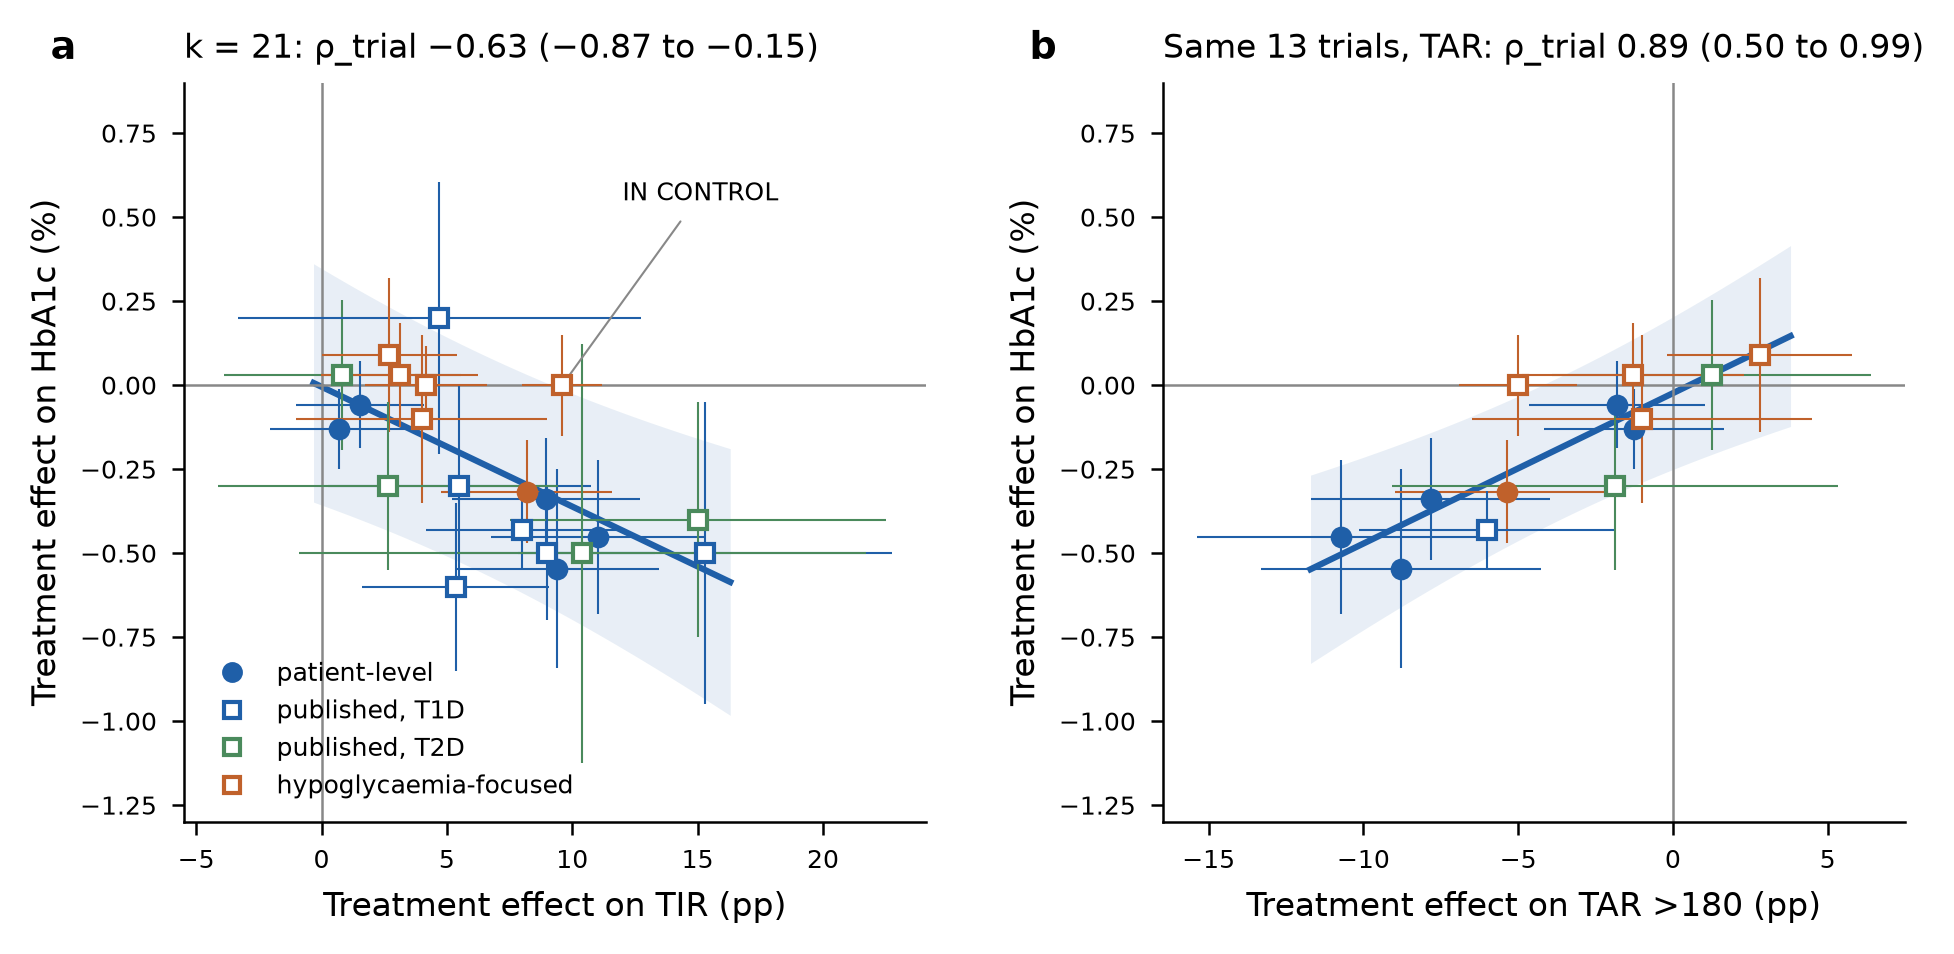
\includegraphics[width=\textwidth]{figures/fig1_trial_level.png}
\caption{\textbf{Treatment effects on time in range and on time above range against treatment effects on
HbA\textsubscript{1c}.} (A) All 21 primary trials. Filled circles are trials contributing individual patient
data, open squares published aggregate effects; orange marks trials whose primary objective was reduction of
hypoglycaemia. Bars are 95\% CIs. The line and band are the random-effects meta-regression with its 95\%
prediction interval. IN CONTROL is labelled as the most influential trial. (B) The same model fitted to time
above range on the 13 trials reporting it. pp = \pp.}
\end{figure}

\begin{figure}[htbp]
\centering
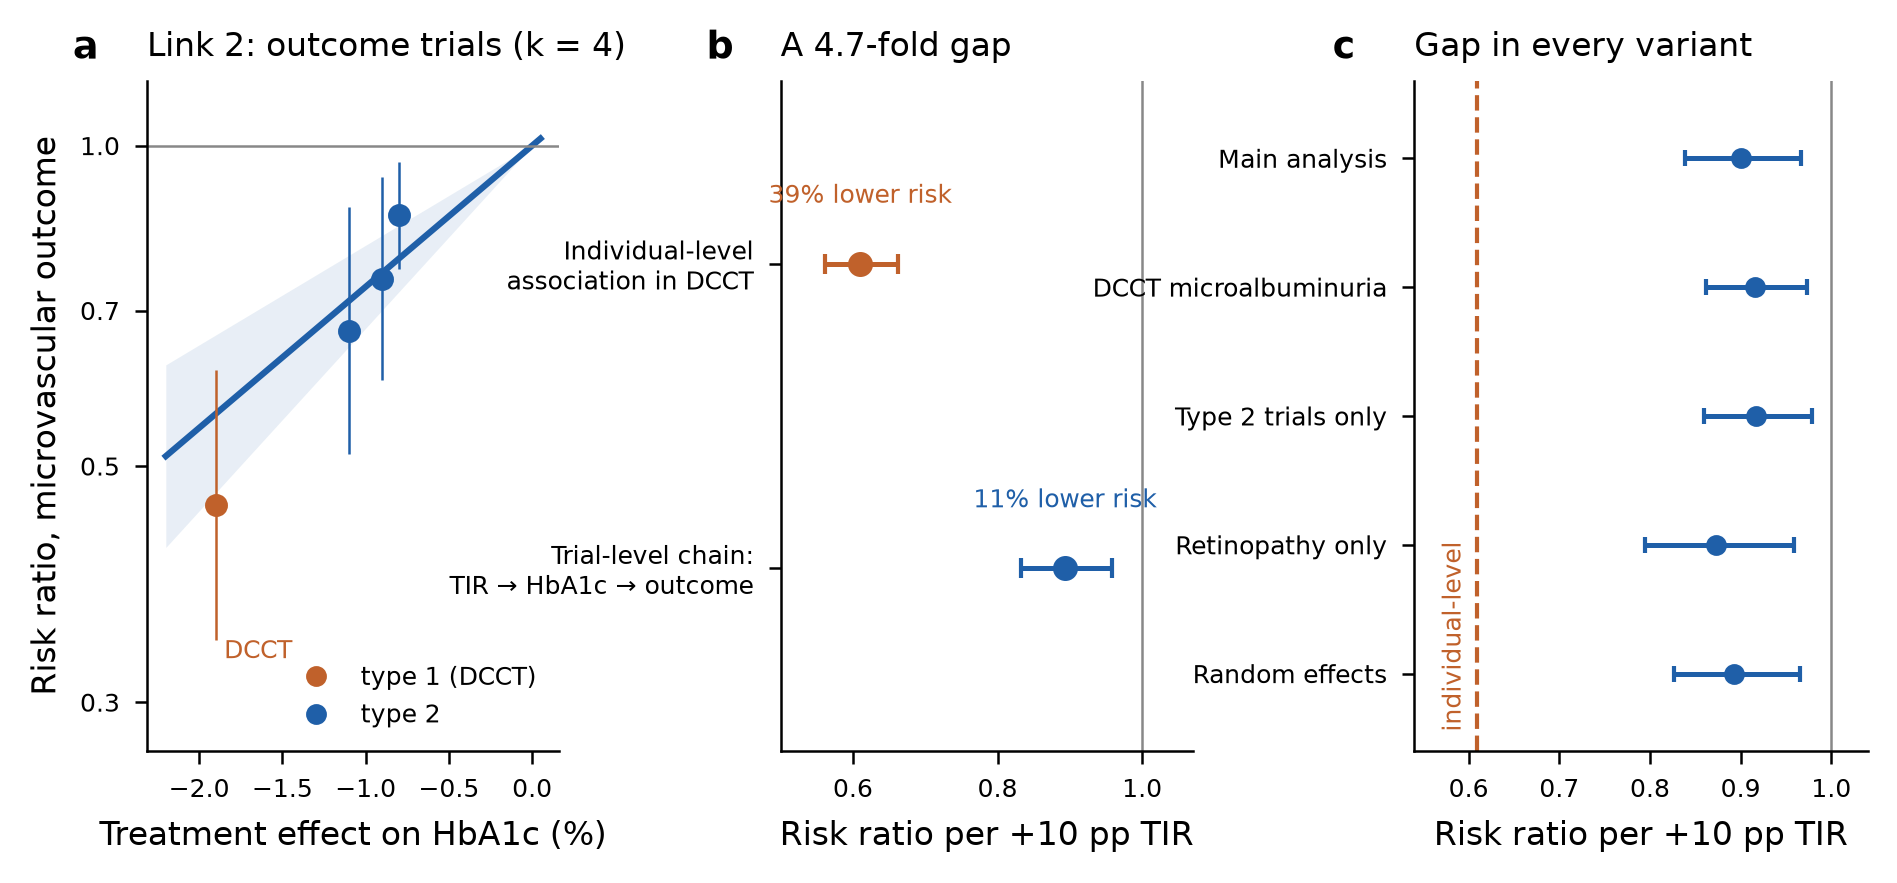
\includegraphics[width=\textwidth]{figures/fig2_chain.png}
\caption{\textbf{The surrogacy chain to microvascular outcomes.} (A) Link 2: log risk ratio for the
microvascular outcome against achieved between-group HbA\textsubscript{1c} difference in four glycaemic-control
trials, fitted through the origin (band is the 95\% CI of the slope). (B) The interventional estimate implied
by the chain compared with the published individual-level association, both expressed per $+10$ \pp{} time in
range. (C) The same comparison under five variants of the analysis; the dashed line marks the individual-level
estimate.}
\end{figure}

\clearpage
\bibliographystyle{unsrtnat}
\bibliography{references}

\end{document}
